\subsection{Modelo conceptual}

\subsubsection{Diagrama de clases}

En este modelo se podrá visualizar los conceptos más importantes del sistema. A estos conceptos los llamaremos clases, las cuales tienen atributos que caracterizan a dicho concepto. También mostraremos las relaciones entre estas clases, el tipo de relación (uno a uno, uno a muchos, muchos a muchos, etc), el rol de cada clase en la relación, clases de asociación en la relación y los casos de herencia entre clases.
Luego, usaremos OCL para realizar restricciones de instanciación de las clases.

En este diagrama mostramos la información que almacena el sistema:
\begin{itemize}
\item Historial de pedidos realizados por un cliente.
\item Historial de pedidos realizados por un local.
\item Información de cada pedido: estado, fecha de entrega, método de pago, productos pedidos y su cantidad, depósito que atendió el pedido, etc.
\item Configuración de los umbrales de cada depósito (por producto).
\item Stock reservado y disponible de cada depósito (por producto).
\item Historial de penalización de cada usuario.
\item Datos personales de cada usuario.
\item Datos de cada depósito.
\end{itemize}

A continuación mostraremos el diagrama de clases y las restricciones OCL realizadas:

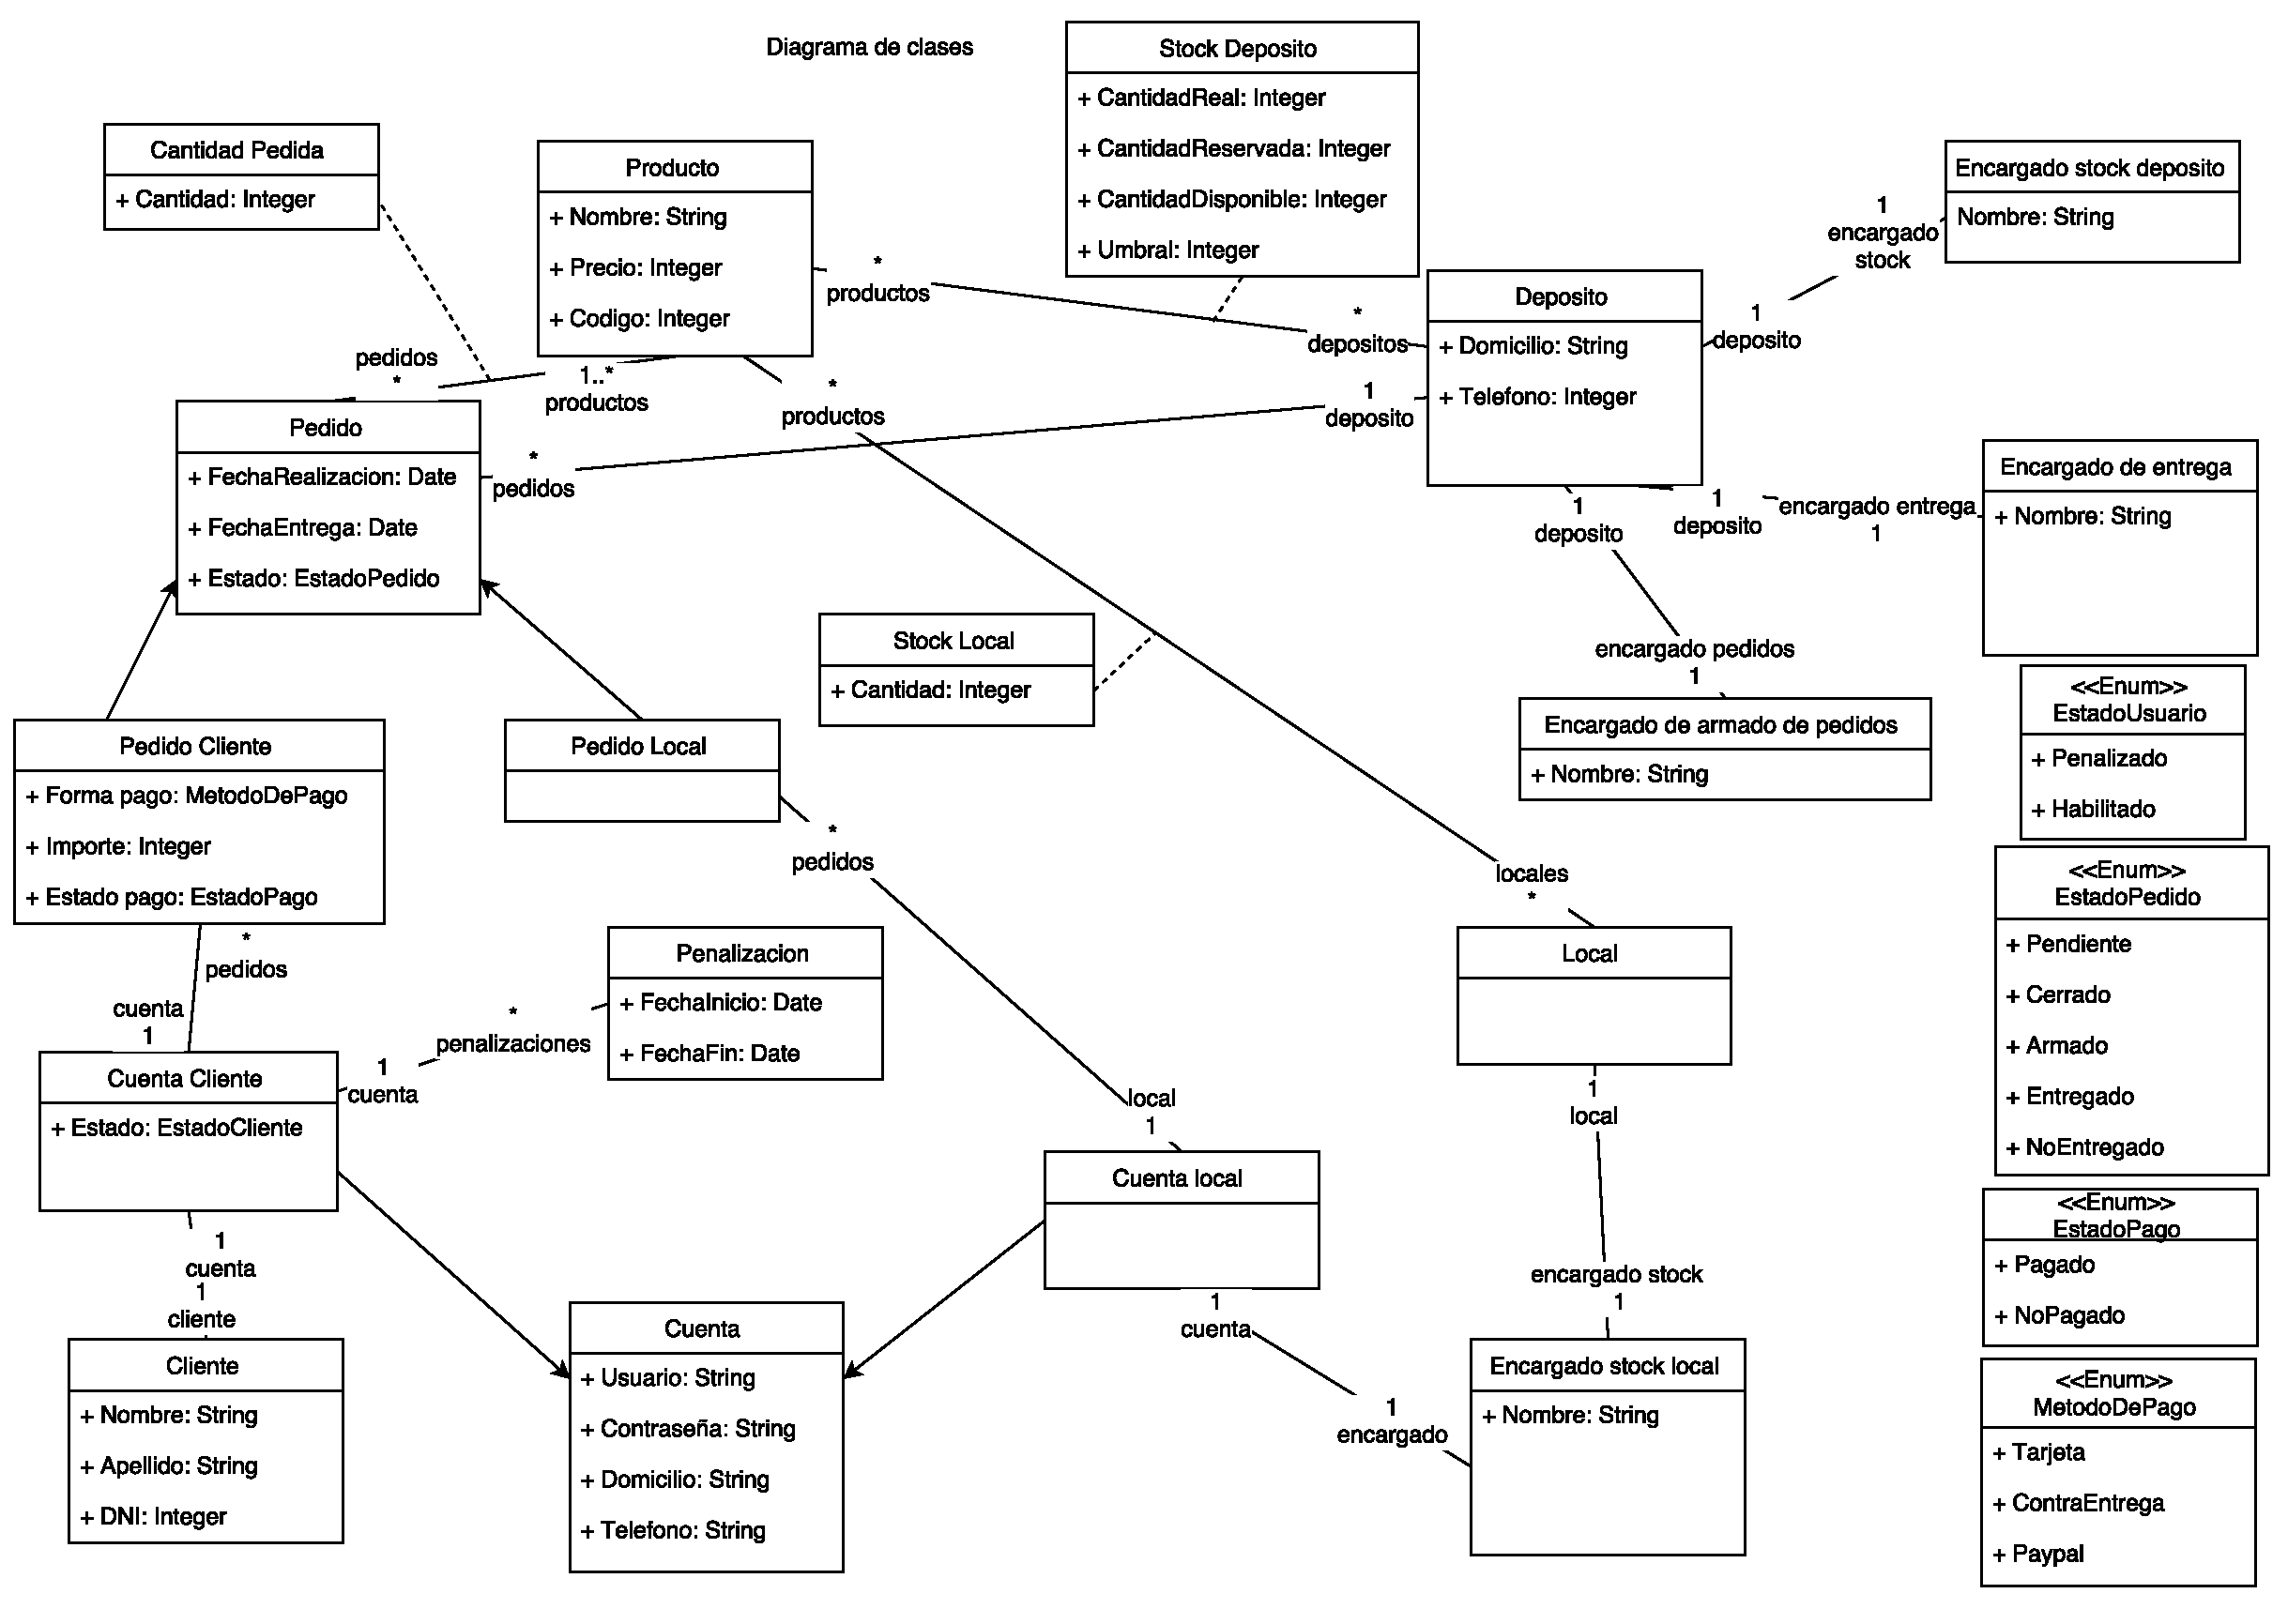
\includegraphics[scale=0.5, angle=90]{secciones/diagramaClases}
\newpage

\subsubsection{Restricciones OCL}

\begin{enumerate}
    \item Los clientes solo pueden tener un pedido activo a la vez.

    \begin{center}
    \begin{tabular}{p{0.2\textwidth} p{0.8\textwidth}}
        \textsc{Contexto} & Cuenta Cliente \\
        \textsc{Invariante} & \texttt{self.pedidos->select(p | p.Estado =
        Pendiente or p.Estado = Cerrado or p.Estado = Armado)->size() <= 1} \\
    \end{tabular}
    \end{center}

    \item Los locales solo pueden tener un pedido de reposición de stock activo a la vez.

    \begin{center}
    \begin{tabular}{p{0.2\textwidth} p{0.8\textwidth}}
        \textsc{Contexto} & Cuenta local \\
        \textsc{Invariante} & \texttt{self.pedidos->select(p | p.Estado =
        Pendiente or p.Estado = Cerrado or p.Estado = Armado)->size() <= 1} \\
    \end{tabular}
    \end{center}

    \item Calculo de la cantidad disponible de un producto en el stock de un deposito.

    \begin{center}
    \begin{tabular}{p{0.2\textwidth} p{0.8\textwidth}}
        \textsc{Contexto} & Stock Depósito \\
        \textsc{Invariante} & \texttt{self.CantidadDisponible = self.CantidadReal - self.CantidadReservada} \\
    \end{tabular}
    \end{center}

    \item La cantidad reservada de un producto en un deposito es igual a la suma de la cantidad pedida de ese producto en los pedidos activos realizados a dicho deposito.

    \begin{center}
    \begin{tabular}{p{0.2\textwidth} p{0.8\textwidth}}
        \textsc{Contexto} & Depósito \\
        \textsc{Invariante} & \texttt{self.Stock Deposito->forAll(sd | sd.CantidadReservada = self.pedidos->select(pe | pe.productos->exists(sd.Producto) and (pe.Estado = Pendiente or pe.Estado = Cerrado or pe.Estado = Armado))->collect((pe, sd.Producto).Cantidad)->sum()} \\
    \end{tabular}
    \end{center}
    
        \item La fecha de inicio de una penalización es anterior a su fecha de finalización.

    \begin{center}
    \begin{tabular}{p{0.2\textwidth} p{0.8\textwidth}}
        \textsc{Contexto} & Penalización \\
        \textsc{Invariante} & \texttt{self.FechaInicio <\ self.FechaFin} \\
    \end{tabular}
    \end{center}

    \item No puede haber pedidos por parte de un cliente con fecha dentro del
    rango de alguna penalización de esa cuenta.

    \begin{center}
    \begin{tabular}{p{0.2\textwidth} p{0.8\textwidth}}
        \textsc{Contexto} & Cuenta cliente \\
        \textsc{Invariante} & \texttt{self.pedidos->forAll(p |
        self.penalizaciones->forAll(pen | p.Fecha < pen.FechaInicio or p.Fecha > pen.FechaFin)} \\
    \end{tabular}
    \end{center}

    \item Los períodos de las penalizaciones de un cliente no pueden solaparse.

    \begin{center}
    \begin{tabular}{p{0.2\textwidth} p{0.8\textwidth}}
        \textsc{Contexto} & Cuenta cliente \\
        \textsc{Invariante} & \texttt{self.penalizaciones->forAll(p1, p2 |
        p1.FechaFin < p2.FechaInicio or p1.FechaInicio > p2.FechaFin)} \\
    \end{tabular}
    \end{center}

    \item Los productos de los pedidos atendidos por un depósito tiene que
    estar en el catálogo de dicho depósito.

    \begin{center}
    \begin{tabular}{p{0.2\textwidth} p{0.8\textwidth}}
        \textsc{Contexto} & Pedido \\
        \textsc{Invariante} &
        \texttt{self.deposito.productos->includesAll(self.productos)} \\
    \end{tabular}
    \end{center}


    \item Los pedidos de los locales no pueden estar marcados como no
    entregados.

    \begin{center}
    \begin{tabular}{p{0.2\textwidth} p{0.8\textwidth}}
        \textsc{Contexto} & Pedido local \\
        \textsc{Invariante} & \texttt{self.Estado <>\ NoEntregado} \\
    \end{tabular}
    \end{center}
    
    \item Definición de cuando un cliente esta penalizado.

    \begin{center}
    \begin{tabular}{p{0.2\textwidth} p{0.8\textwidth}}
        \textsc{Contexto} & Cuenta cliente \\
        \textsc{Invariante} & \texttt{if (self.penalizaciones->exists(p | p.FechaInicio <= now() <= p.FechaFin) then self.Estado = Penalizado else self.Estado = Habilitado endif)} \\
    \end{tabular}
    \end{center}
    
    \item Calculo del importe de un pedido.

    \begin{center}
    \begin{tabular}{p{0.2\textwidth} p{0.8\textwidth}}
        \textsc{Contexto} & Pedido Cliente \\
        \textsc{Invariante} & \texttt{self.Importe = self.Cantidad\ Pedida->collect(cp | cp.Cantidad * cp.Producto.Precio)->sum()} \\
    \end{tabular}
    \end{center}
    
     \item La fecha de entrega de un pedido debe ser igual o posterior a la fecha en la que se realizo el pedido.

    \begin{center}
    \begin{tabular}{p{0.2\textwidth} p{0.8\textwidth}}
        \textsc{Contexto} & Pedido \\
        \textsc{Invariante} & \texttt{self.FechaRealizacion <= self.FechaEntrega} \\
    \end{tabular}
    \end{center}
    
    \item Los pedidos entregados siempre son pagados.
    
    \begin{center}
    \begin{tabular}{p{0.2\textwidth} p{0.8\textwidth}}
        \textsc{Contexto} & Pedido Cliente \\
        \textsc{Invariante} & \texttt{self.Estado == ``Entregado'' implies self.Estado pago == ``Pagado''} \\
    \end{tabular}
    \end{center}
    
    \item Los pedidos que se pagan online con tarjeta o por Paypal siempre se marcan como pagados.
    
    \begin{center}
    \begin{tabular}{p{0.2\textwidth} p{0.8\textwidth}}
        \textsc{Contexto} & Pedido Cliente \\
        \textsc{Invariante} & \texttt{(self.Forma pago == ``Tarjeta'' or self.Forma pago == ``Paypal'') implies self.Estado pago == ``Pagado''} \\
    \end{tabular}
    \end{center}
    
    \item El stock reservado no puede superar al stock real del deposito.
    
    \begin{center}
    \begin{tabular}{p{0.2\textwidth} p{0.8\textwidth}}
        \textsc{Contexto} & Stock Deposito \\
        \textsc{Invariante} & \texttt{self.CantidadReservada <= self.CantidadReal} \\
    \end{tabular}
    \end{center}
    
    \item Los pedidos se entregan, a lo sumo, siete días después de haber sido realizados.
    
    \begin{center}
    \begin{tabular}{p{0.2\textwidth} p{0.8\textwidth}}
        \textsc{Contexto} & Pedido \\
        \textsc{Invariante} & \texttt{self.FechaEntrega - self.FechaRealizacion <= 7} \\
    \end{tabular}
    \end{center}

\end{enumerate}

\subsubsection{Generación de los reportes de ventas}

Para mostrar como se podría generar un reporte de ventas en este modelo conceptual presentamos tres ejemplos:

\begin{itemize}
\item \textbf{Productos mas vendidos}: Primero, tomamos los objetos de la clase ``Cantidad Pedida'' y, para cada producto, sumamos el valor del campo ``Cantidad'' de los objetos de la clase ``Cantidad Pedida'' que estén relacionados con el objeto de la clase ``Producto'' que representa al producto en cuestión. Luego, ordenamos esta lista de forma decreciente.
\item \textbf{Depósitos con mas pedidos}: Dado un deposito podemos obtener todos los pedidos realizados a este mediante su relación con la clase ``Pedido''. Luego, haciendo \textit{size()} al conjunto obtenido por esta relación podemos obtener la cantidad de pedidos de cada deposito. Así podemos armar un lista, con la cantidad de pedidos de cada deposito y, luego, ordenarla de forma decreciente.
\item \textbf{Métodos de pago}: Dado todo el conjunto de instancias de ``Pedido Cliente'', filtramos por cada método de pago ofrecido a los pedidos cuyo campo ``Forma de pago'' se corresponda con el método de pago deseado y, luego, contamos cuantas instancias tenemos para cada uno de los métodos.
\end{itemize}

\subsubsection{Trazabilidad}
A continuación listamos los requerimientos que se modelan con este diagrama.

\begin{itemize}
\item \textbf{Agregar depósitos al sistema:} se agrega una nueva  Clase Deposito 
\item \textbf{Cerrar un pedido desde la pagina web:} el objeto pedido cambia su estado a cerrado
\item \textbf{Tomar productos del pedido => Notificar pedido armado:}  El estado del pedido cambia a armado
\item \textbf{Configurar umbrales por producto en el sistema:}  stockDeposito.umbral = umbral configurado
\item \textbf{Incrementar stock cuando recibo reposición del proveedor:}  stockDeposito.cantidadReal se le incrementa el stock que se pidió
\item \textbf{Coordinar fecha de entrega:}  Pedido.fechaDeEntrega $=$ fecha que el cliente acuerda
\item \textbf{Se puede consultar los registros de las ventas:}  \textbf{informe}
\item \textbf{Se puede configurar los parámetros del reporte:}  \textbf{informe}
\item \textbf{Mantener listado de productos comprados:}  Pedido.productos si Pedido.estado = Pagado
\item \textbf{Mantener información de los medios de pagos utilizados:}  
\item \textbf{Los locales puedan registrarse:}  PedidoCliente.metodoDePago
\item \textbf{Los locales pueden modificar los pedidos no cerrados:}  si Pedido.estado != Cerrado entonces se modifican las relaciones con productos
\item \textbf{Los clientes pueden modificar los pedido no cerrados:}  si Pedido.estado != Cerrado entonces se modifican las relaciones con productos
\item \textbf{Un cliente pueda registrarse:}  se crea un nuevo objeto CuentaCliente
\item \textbf{Un cliente pueda seleccionar la fecha de entrega:}  Pedido.fechaDeEntrega = fecha que el cliente acuerda
\item \textbf{Un cliente pueda ingresar sus datos de contacto:}  atributos de clase Cuenta
\item \textbf{Reservar stock:}  StockDeposito.cantidadReservada igual al stock reservado
\item \textbf{Consultar pedidos armados:}  se muestran los pedidos tal que Pedido.estadoPedido = Armado
\item \textbf{Seleccionar pedido entregado:}   se modifica Pedido.estadoPedido = Entregado
\item \textbf{El cliente pago en contra-entrega => se notifica pago a contra-entrega:}    se modifica Pedido.estadoPedido = Pagado
\item \textbf{El cliente pago desde la pagina => se notifica el pago online:}  se modifica Pedido.estadoPedido = Pagado
\item \textbf{Llevar el conteo en base a los pedidos realizados de cuantos productos quedan:}  StockDeposito.cantidadDisponible
\item \textbf{Mantener historial de pedidos entregados y no entregados de un cliente:}  Instancias de la clase Pedido asociadas con una instancia de la clase Cuenta
\item \textbf{Rechazar pedido durante un tiempo:}  clase Penalizacion
\item \textbf{Pedido llega a la casa del cliente:}  PedidoCliente.estadoPedido = Entregado
\item \textbf{Cliente pague el pedido:}  PedidoCliente.estadoPedido = Pagado
\item \textbf{Ofrecer pago con PayPal:}  PedidoCliente.metodoDePago = PayPal
\item \textbf{Ofrecer pago con credito:}  PedidoCliente.metodoDePago = Tarjeta
\item \textbf{Ofrecer pago con debito:}  PedidoCliente.metodoDePago = Tarjeta
\item \textbf{Ofrecer pago con efectivo:}  PedidoCliente.metodoDePago = ContraEntrega
 
\end{itemize}

\newpage